% --
% raw audio

\section{Raw Audio Waveforms}\label{sec:raw_audio}\label{sec:signal_raw}
Physical acoustic waves can be recorded by microphones, translating mechanical vibrations to electrical signals. 
Those electrical signals are further stored in so called \emph{waveform files} or \emph{audio files}.

First it is to mention that waveform files are stored with a specific audio format, for example \texttt{.wav} files, using parameters such as bit resolution, e.g. \SI{32}{\bit} floating point, and most importantly a sample rates $f_s$. 
The sample rate tells, which frequency range of the continuous acoustic waves form is possible to store in a discrete representation.
This is restricted by the Nyquist-Shannon sampling theorem, where the maximal frequency of the signal $f_{x_{max}}$ should not be larger than the half of the sampling frequency: 
\begin{equation}\label{eq:signal_raw_nyquist}
  f_{x_{max}} < \frac{fs}{2}
\end{equation}
to prevent aliasing effects.

That is the reason, why a compact disc (CD) format has a sampling frequency of \SI{44.1}{\kilo\hertz} resulting in a maximum signal frequency of \SI{22.05}{\kilo\hertz}.
Using the fact that usually humans do not hear above \SI{20}{\kilo\hertz} frequencies.
However it is also possible to go far beyond those \SI{44.1}{\kilo\hertz}, for instance used in telephone systems, where the sampling rate is \SI{8}{\kilo\hertz}.
It is possible to reduce the sampling rate, because voice does not need such a high sampling frequency, as for instance music does, to have sufficient quality and being understandable.

With the sampling frequency known, a discrete time signal of an audio recording $x \in \R^n$ can be expressed in vector notation:
\begin{equation}\label{eq:signal_raw_x}
  x = [x_1,\, x_2,\, \dots,\, x_n]^T
\end{equation}
with a total number of samples $n$.

The audio files provided in the speech command dataset \cite{Warden2018} used for the experiments in \rsec{exp}, are recorded with a sampling rate of \SI{16}{\kilo\hertz}, which is totally enough for human speech.
Further those audio files in the speech command dataset usually have a time length of \SI{1}{\second}.
The author of this thesis recorded his own speech commands with one example of each command shown in \rfig{raw_audio_my}.

\begin{figure}[!ht]
  \centering
    \subfigure[left]{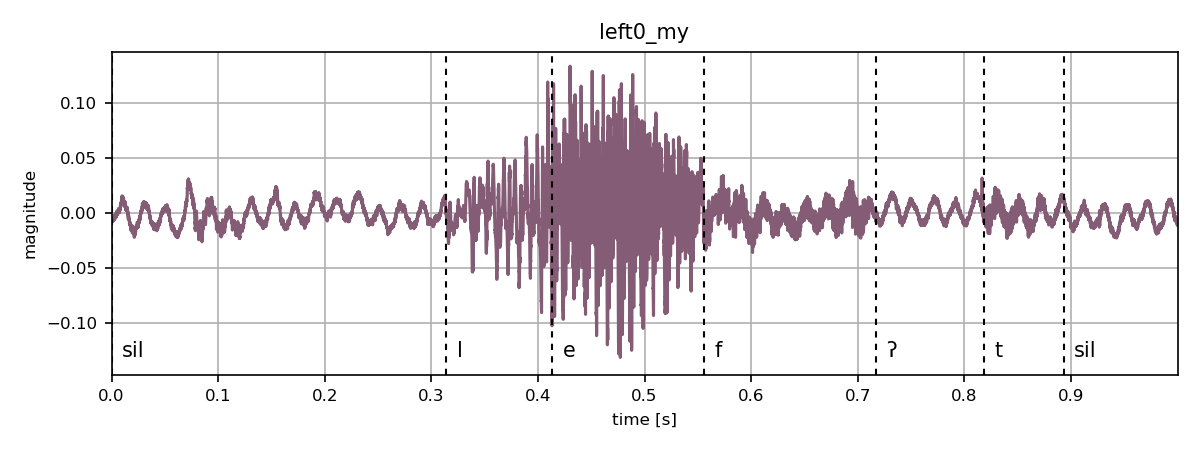
\includegraphics[width=0.45\textwidth]{./3_signal/figs/signal_raw_left0_my}}
    \subfigure[right]{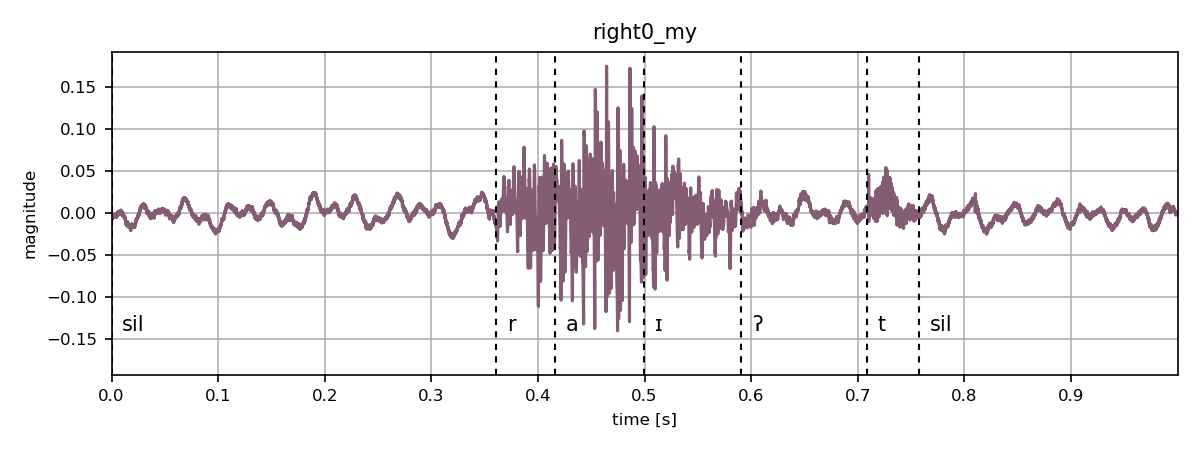
\includegraphics[width=0.45\textwidth]{./3_signal/figs/signal_raw_right0_my}}
    \subfigure[up]{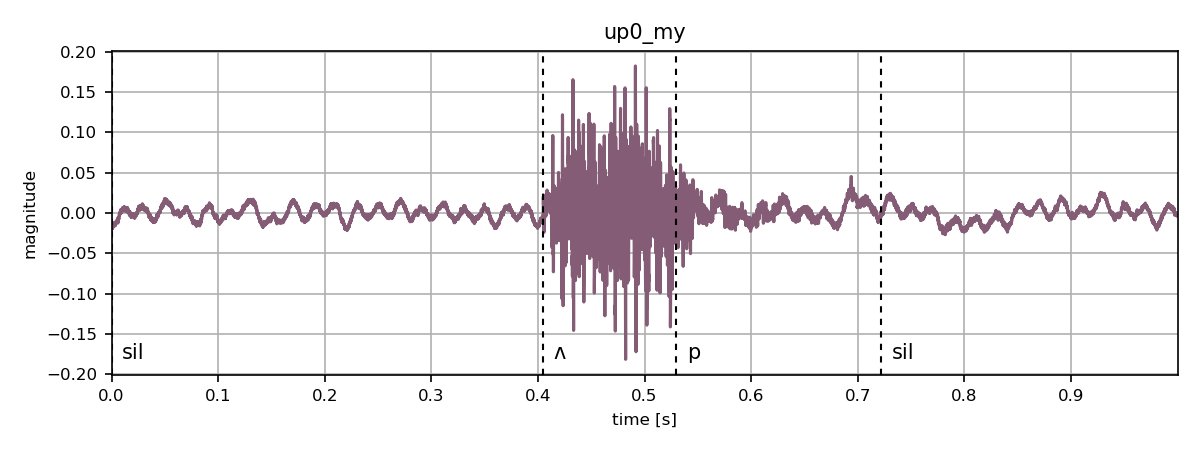
\includegraphics[width=0.45\textwidth]{./3_signal/figs/signal_raw_up0_my}}
    \subfigure[down]{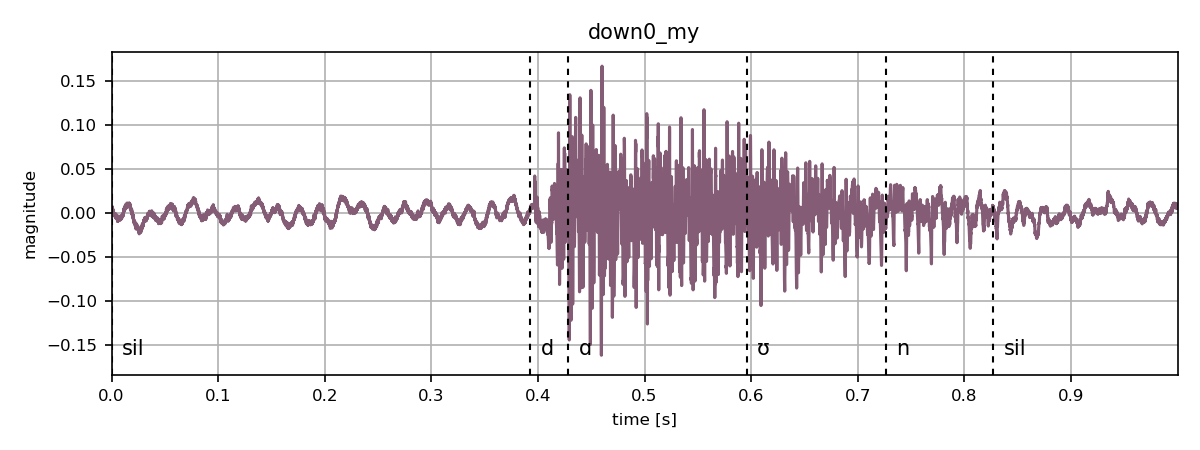
\includegraphics[width=0.45\textwidth]{./3_signal/figs/signal_raw_down0_my}}
    \subfigure[go]{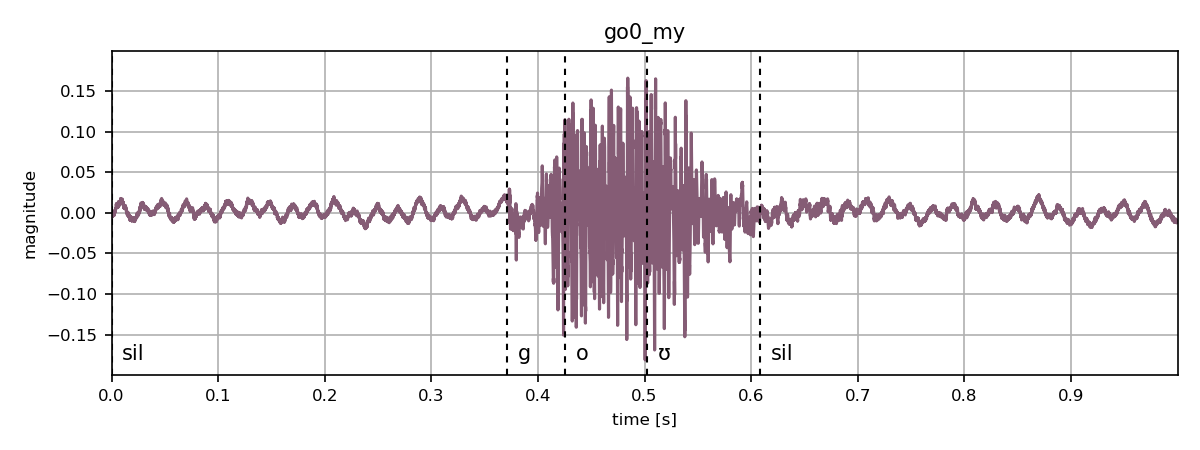
\includegraphics[width=0.45\textwidth]{./3_signal/figs/signal_raw_go0_my}}
  \caption{Raw audio waveform files, recorded and annotated by the author of this thesis with $f_s=\SI{16}{\kilo\hertz}$ and a simple consumer lavalier microphone.}
  \label{fig:raw_audio_my}
\end{figure}
\FloatBarrier
\noindent
From the raw audio files with annotations, one can observe that and estimate how long a speech command may take in terms of time and see that usually a whole second is too much for a single speech command.
Of course one can pronounce words longer or shorter, but usually in commanding something it is preferred to speak short well pronounced.
If a time interval of \SI{500}{\milli\second} is used to capture a speech command (this time interval is used in the feature extraction for the machine learning), it might happen that not every phonetic letter of the words are captured. 
For instance this might happen often for words with glottal stops before consonants, as the phoneme \enquote{t} in \enquote{left} or \enquote{right}.
So the input features may only have information of the first phonetics, for example \enquote{lef} or \enquote{righ}, but since Key Word Spotting is restricted in its vocabulary, it should not be a problem in distinguishing these two words when using a time interval of \SI{500}{\milli\second}.

Another important point is to detect where the onset of the speech command is located on the time axis. It is easy to see in \rfig{raw_audio_my} where the words are starting, but usually not all recordings are as clean as those.
There might be a huge noise level or background noise and it is difficult to find the right onset position for the \SI{500}{\milli\second} time interval with the \SI{1}{\second} recordings.
For this Question to answer, it is postponed to the next sections on feature extraction.
At last it should be noted, that the value range in the y-axis of audio recordings strongly depends on the microphone, amplifiers and post processing.
Therefore it is strongly recommended to normalize all recordings to a defined value range, with for instance the infinity norm, so that the maximum or minimum value is $-1$ or $1$ and the signal range is between $[-1, 1]$.